\chapter{VISUAL SOLUTIONS FOR DOI INTERPRETATION}
\label{chap:DOIVis}
In this chapter we discuss the possible visual interpretations for DOI data. AOI is image-space counter part of DOI. Although plethora of visual solutions exist for AOI~\cite{Bla14}, three distinct properties of DOIs prohibit them to interpret DOI data. First, DOI data has volumes and multiple granularities. Second, DOI data deals with data attributes. Third, DOI data supports different range of analysis questions possible compared to AOI data. 

Thus, DOI visualizations should allow analysts to explore DOI data at many levels of detail, including multiple temporal scales (e.g., seconds vs. minutes) and data granularities (e.g., individual vs. categories of DOIs).  DOI attributes should be shown visually and queried flexibly to allow analysts to detect correlations between a user's interest in data and that data's properties. Attributes should be used to deal with the scale of the data by allowing users to filter, highlight, and aggregate data with specific attribute values. Finally, visualizations need to support the DOI analysis tasks. 



\section{Existing Visualizations for Eye-tracking Data}
\label{sec:ClassicVisualization}
In this section, we discuss existing visualization techniques for eye-tracking data. Specifically, we will focus on three basic visualization techniques: Heatmap, Scanpath, and Scarfplot. %Moreover, we will briefly discuss about three advanced techniques : AOI-river, Transition Matrices, and Directed graphs.

\subsection{Heatmap}
Heatmap visualization contains a 2D matrix where each cell is assigned a color. The color used in the cell represent value of the cell. Multiple color schemes exist to represent color to value. The most popular color scheme is the 'Rainbow' color scheme. In rainbow color scheme, 'red' represents maximum and 'violet' represents minimum. Many heatmap visualizations also use green or blue for minimum. However, rainbow color scheme lacks perceptual ordering, and not sensitive small value changes~\cite{borland2007rainbow}. Hence, visualization researchers consider rainbow color scheme as misleading. Many heatmaps use color scales such as gray-scale, heated-object, and linearized optimal scale~\cite{silva2007there}. Figure~\ref{fig:heatmapsExample} depicts an example of heatmaps with three different color schemes. 

\begin{figure}[htbp]
  \centering
  \includegraphics[width=\linewidth]{images/heatmapsExample.eps}
  \caption{Heatmap visualization with three different color schemes: (a) rainbow, (b) gray-scale, and (c) heated object.}
	\label{fig:heatmapsExample}
\end{figure}



\subsection{Scanpath}
A scanpath visualization depicts transitions among multiple entities over time. Scanpath visualization either show temporal information in a linear scale or discard temporal information. For example, we encode transitions among five entities $e_1 \rightarrow e_2\rightarrow e_3\rightarrow e_4\rightarrow e_5\}$ with scanpath visualization. Figure~\ref{fig:scanpathExample}(a) portray all transitions among entity to entity. Such techniques require a layout with minimal crossing among transitions. However, it produces a compact visualization. Again, in Figure~\ref{fig:scanpathExample}(b), all entities lie vertically and are connected with a horizontal line to show temporal information. For depicting a transition between $e_1$ and $e_2$, we place transition markers (e.g. a circle) along their horizontal lines. Then, we connect the markers with transition encoding (e.g. an arrow). The latter technique is more suitable for following transitions. However, it takes more space than the former version. 

\begin{figure}[htbp]
  \centering
  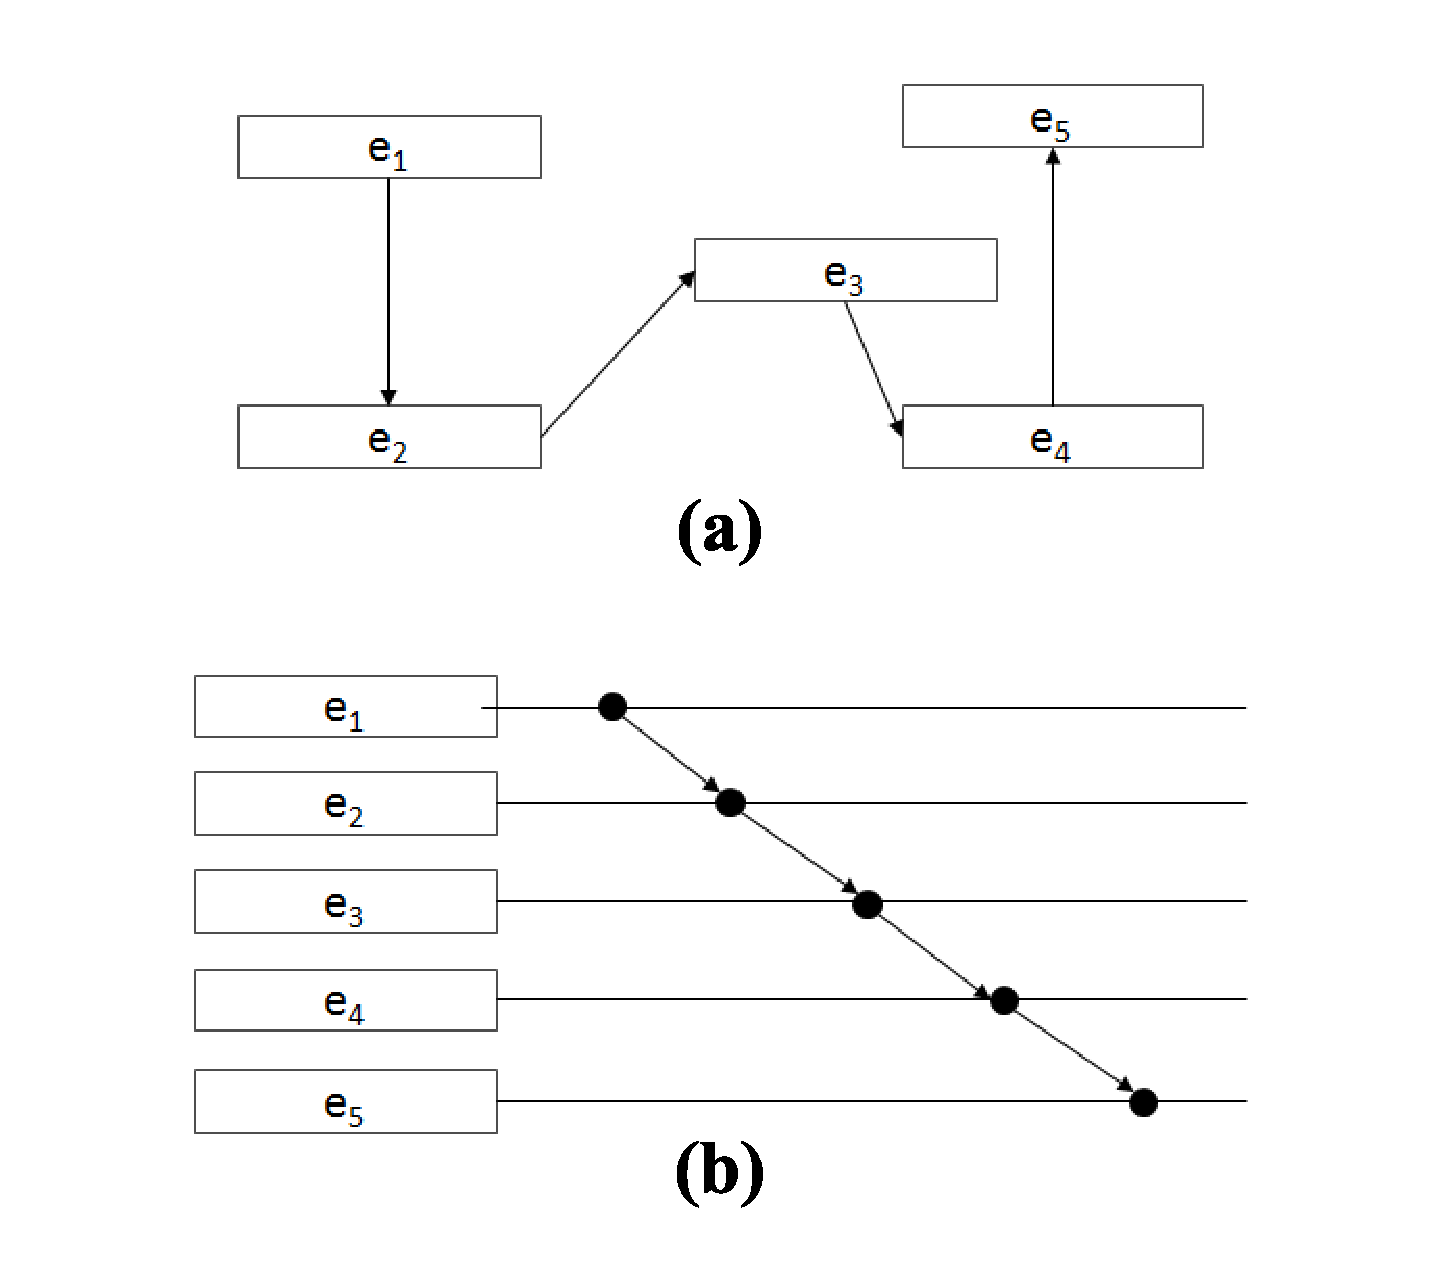
\includegraphics[width=\linewidth]{images/scanpathExample.eps}
  \caption{Scanpath visualization (a) without explicit temporal information, (b) with temporal transitions.}
	\label{fig:scanpathExample}
\end{figure}

\subsection{Scarfplot}
In a scarplot technique, visual entities are joined as multiple tapes known as scarflines~\cite{richardson2005looking}. The entities may have different width in tapes. The width usually represent data value (e.g. intensity). Figure~\ref{fig:scarfplotExample} demonstrate an example of transitions viewing pattern for two users. $User_1$ viewed entities $e_1, e_2, e_3, e_4,e_5$ and $User_2$ viewed $e_6, e_7$. Scarfplot technique is useful for finding pattern among multiple sets of data. 
\begin{figure}[htbp]
  \centering
  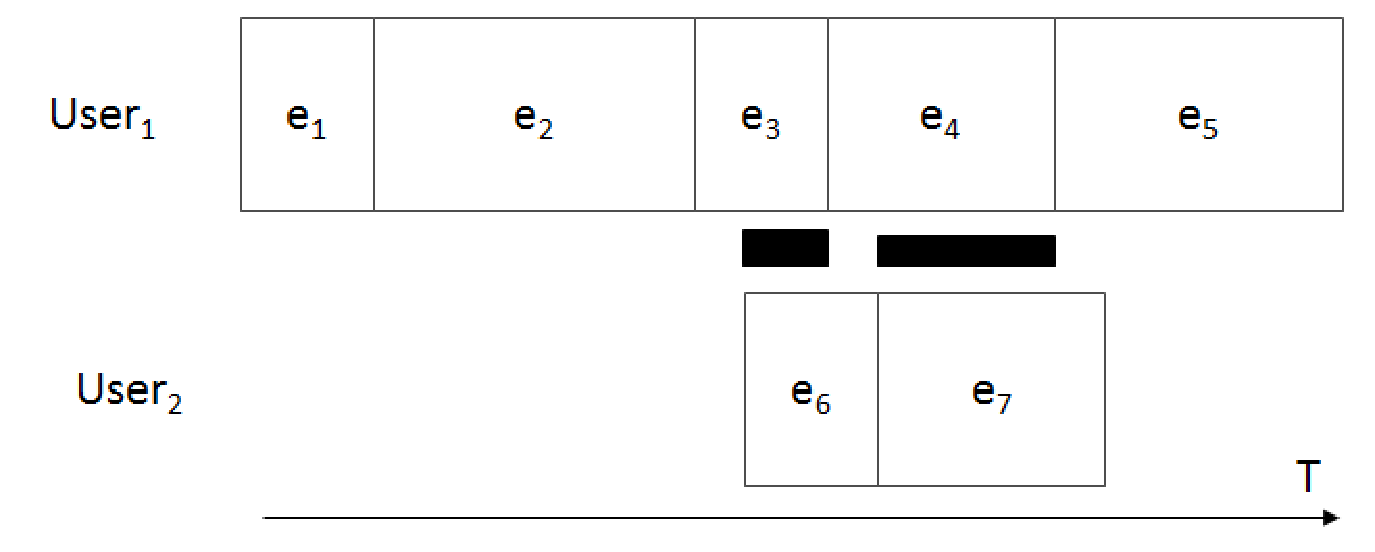
\includegraphics[width=\linewidth]{images/ScarfplotExample.eps}
  \caption{An example of Scarfplot visualization. }
	\label{fig:scarfplotExample}
\end{figure}

\section{Case Studies}
In this section, we discuss our implementation of four DOI analysis visualizations: heatmap, scanpath, scarfplot, and stacked glyph-plot. We developed these visualizations based on collected DOI data from experiments in Chapter~\ref{chap:CaseStudies}. Specifically, we developed  for the experiment described in Section~\ref{sec:ExperimentIMDB}. Next, we developed another heatmap for experiment described in Section~\ref{sec:ExperimentArchitecture}, and a stacked glyph plot for the experiment described in Section~\ref{sec:ExperimentConstruction}. We discuss more about them below. 

\subsection{DOI Vis for Tracking Data Consumption Experiment}
We already discussed about the data collection and instrumentation methods about the tracking data consumption experiment in Section~\ref{sec:ExperimentIMDB}. To analyze the data collected from this experiment, we developed three visualizations: heatmap, scanpath, and scarfplot. 

First, we developed a time-annotated heatmap (Figure~\ref{fig:HeatmapIMDB}) where each cell's color represents viewing score (i.e. viewing intensity). We chose the grayscale color scheme to render the heatmap where black represents maximum and white represents minimum. In our visualization, we facilitate interaction of panning to view time-based data. For facilitating comparison, we allowed rendering user data views side by side. 
\begin{figure}[htb]
  \centering
	\includegraphics[width=0.6\linewidth]{images/HeatmapIMDB.eps}
  \caption{Heatmap of real DOI data. User data is shown separately. DOI-rows are scaled vertically to make DOIs viewed often more salient. DOIs are ordered by viewing amount; those beyond a threshold are not shown.
  A time-window (white section) helps prioritize which data is shown.}
	\label{fig:HeatmapIMDB}
\end{figure}

Second, we have implemented a scanpath for the same experiment (Figure~\ref{fig:ScanpathsIMDB}). Unlike heatmap, we considered every DOI is viewed when its viewing score crossed a threshold value (e.g. 0.75). Then, we connected the DOI cell to render the scanpath. The scanpath rendering had two versions: juxtaposed (Figure~\ref{fig:ScanpathsIMDB}(left)) and superpositioned(Figure~\ref{fig:ScanpathsIMDB}(right)). We applied a string edit-distance clustering over the vertical sequence of DOIs to reduce cluttering. 
\begin{figure}[!htb]
  \centering
  \includegraphics[width=0.75\linewidth]{images/ScanpathsIMDB.eps}
  \caption{Scanpaths of real DOI data. (left) Data is shown separately for each user. Depicted DOIs are the same for all four users, enabling the comparison of the scanpath profile; the top two users viewed simialr data. (right) Users' data are shown next to each other for each DOI; we notice that the four users cluster into two pairs, based on their interests.}
	\label{fig:ScanpathsIMDB}
\end{figure}

\begin{figure}
  \centering
  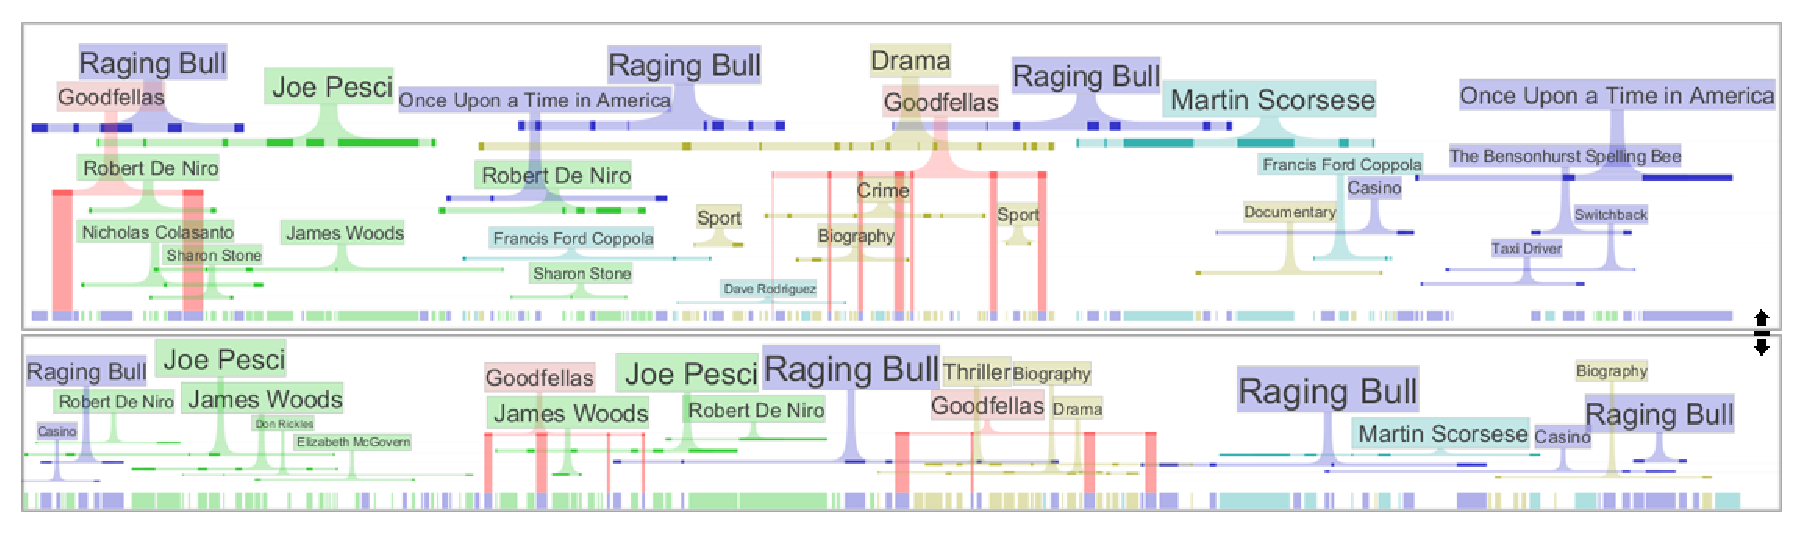
\includegraphics[width=\linewidth]{images/ScarfsIMDB.eps}
  \caption{Re-imagined scarfplots for movie DOI data, sketched for two users. DOI are labeled explicitly, and scaled according to how much they were viewed around particular time-points. Resizing a users' plot vertically would show less or more data. A selection for one user (Goodfellas) is highlighted in all data. }
	\label{fig:ScarfsIMDB}
\end{figure}

Third, we modified the original scarfplot to enable DOI data visualization. We developed a scarfplot with clear labels (Figure~\ref{fig:ScarfsIMDB}. Moreover, the labels are connected with the scarf area on the scarflines. To support multiple granularities, we rendered multiple scarflines to render DOIs clearly. 
%\begin{figure}[htb]
  %\centering
	%\includegraphics[width=0.5\linewidth]{images/MatrixGraphIMDB.eps}
  %\caption{Transition matrix and graph of real DOI data. Both support multiple time-scales by allowing transitions to be defined flexibly, depending on the maximum time allowed to pass between when a first and second object are viewed. The graph shows often viewed objects larger.}
	%\label{fig:MatrixGraphIMDB}
%\end{figure}

\subsection{DOI Vis for Student Learning Experiment}
We developed an interactive heatmap visualization (Figure~\ref{fig:HeatmapArchitecture}) for the student learning experiment from the Section~\ref{sec:ExperimentArchitecture}. In Figure~\ref{fig:HeatmapArchitecture}, we lined up all detected DOIs on the left and their viewing timeline on the right. A sorting option for DOI lineup is also available where we can sort DOIs over first viewed, most viewed or by categories. We collected DOIs of three categories: text, navigation (i.e. buttons, links), and image AOIs. We added selection option where a pop up dialog appears whenever we select any DOI. The pop up dialog generally desribes DOI details and possible image section from the original stimuli. We also enabled the timeline panel to be dragged to have a better view of DOI data. 
\begin{figure}
  \centering
  \includegraphics[width=\linewidth]{images/architecture.eps}
  \caption{Heatmap for architecture }
	\label{fig:HeatmapArchitecture}
\end{figure}

\subsection{DOI Vis for Construction Hazard Detection Experiment}
We implemented a glyph based visualization for hazard detection experiment discussed in Section~\ref{sec:ExperimentConstruction}. The visualization (Figure~\ref{fig:constructionAnalysis}) employs focus+context technique and glyph based solution to handle multiple granularities of DOI data and to handle data attributes. 

Focus+context is an interactive technique which is similar to a technique called overview+detail. Overview+detail have two views of the involving visualization: overview and detail. In the overview view, the whole visualization is viewed with minimal readability and the detail view shows a detail of a part of the context view. On the other hand, focus+context combines the two views in a single coherent view~\cite{spence1982data}. Using such technique will facilitate analyzers to navigate through DOI data. 

On the other hand, a glyph is a small visual object that is discretely placed in visualizations. It is useful to depict data attributes~\cite{borgo2013glyph}. Glyph designing often combines concepts of Gestalt psychology~\cite{kohler1970gestalt}, visual channel selection, and design criteria. For example, if we want to design a glyph for $O = {a_1, a_2}$ where $a_i$ is the $i$th attribute for object $O$. We assume that the attributes are sorted in descending order of importance(i.e. $a_1$ is the most important attribute and $a_2$ is the least). We can assign four visual channels for all the attributes: color, and size. According to pop-out effect of visual channel, color precedes size in importance. Thus, users will be able to detect whether a visual object is red or blue first than whether its big or small. 

A suitable instance of glyph is star-plot. A star-plot contains radially arranged multiple axes (i.e. rays)~\cite{klippel2009star}. Each attribute of involving data element corresponds to a ray. Connecting data points of each ray creates a star-like shape to create such star-plot. Using star-plots for DOI data significantly facilitates handling data attribute. 

In Figure~\ref{fig:StarplotExample}, we describe an example for star plot. Suppose, we want to represent a DOI $D_1=\cup_{1 \leq i \leq N}a_i=v_i $, where $a_i$ represents $i$th attribute and $v_i$ is the value of $a_i$. We entitle a ray for each attribute $a_i$. For $v_i$ we mark a point along the ray for $a_i$. Then, we connect all the line to form a star-like shape.  
\begin{figure}[htbp]
  \centering
  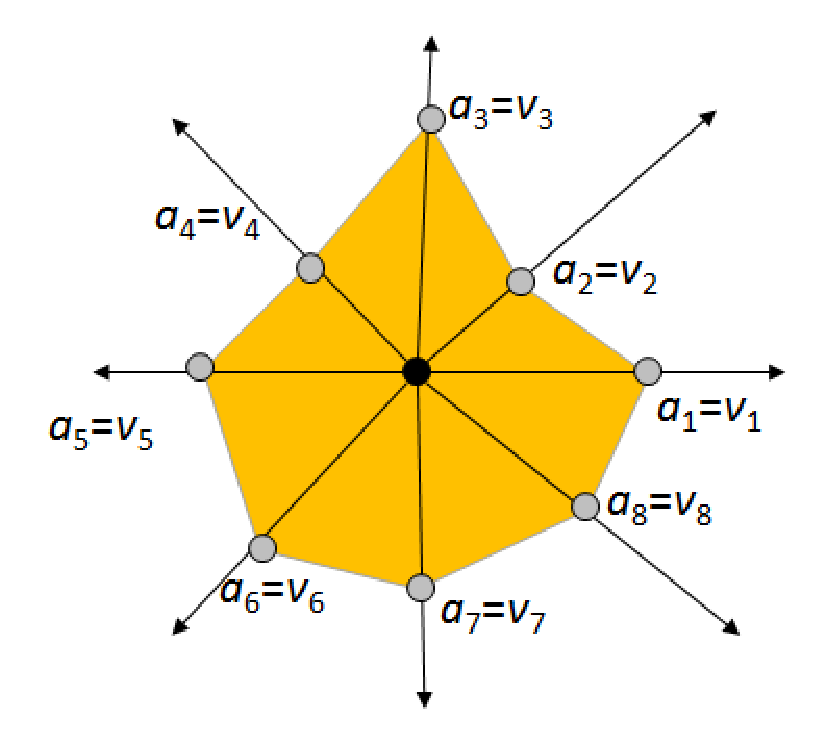
\includegraphics[width=0.5\linewidth]{images/StarplotExample.eps}
  \caption{An example of a Starplot glyph. }
	\label{fig:StarplotExample}
\end{figure}

In Figure~\ref{fig:constructionAnalysis}, we show a glyph for what type of DOI (e.g. worker) it is alongside a star plot over it. We also enabled sorting option based on data attributes. Moreover, we enabled panning and filtering. Again, we used colors to detect whether any hazard was detected over a particular DOI and color coded the hazard. 
\begin{figure}
  \centering
  \includegraphics[width=\linewidth]{images/constructionAnalysis.eps}
  \caption{Stacked Glyph plot for Construction}
	\label{fig:constructionAnalysis}
\end{figure}

\section{A visual design space for DOI analysis}

In this section, we analyze the design space for visual DOI analysis in more detail. Given the scale DOI data and the breadth of DOI tasks, visual encodings should be augmented with interaction capabilities. To ensure that our discussion captures all visual design dimensions, we ground it in Yi's taxonomy of interaction tasks~\cite{Yi07}, which includes seven categories of visual operations: Encoding, Selection, Reconfiguration, Exploration, Abstraction/Elaboration, Filtering, and Connection/Comparison~\cite{Yi07}. We will discuss novel visual solutions by starting from existing AOI visualizations and describing how they may be extended and redesigned to support DOI requirements. 

\subsection{Encoding}
\label{sec:Encoding}
Encoding determines how data should be shown visually~\cite{Yi07}. Encoding design options and requirements of DOI visualizations are detailed below.

\noindent \textbf{Show many DOIs :} AOI visualizations such as scarfplots identify specific AOIs via distinctive colors. This method does not scale to many DOIs, and methods that identify DOIs explicitly (e.g., through a label), such as scan-paths or transition matrices, are likely preferable. 

Also, showing all DOIs viewed in an experiment is not always possible, especially when viewing data from many users. For example, a scanpath of ten users, each having viewed $100$ DOIs would have a thousand rows and be cluttered. One solution is to show only the most viewed DOIs, as done for visualizations shown in Figures~\ref{fig:ScanpathsIMDB},~\ref{fig:ScarfsIMDB},~\ref{fig:HeatmapIMDB},~\ref{fig:HeatmapArchitecture},~\ref{fig:constructionAnalysis} and to alot DOI space that is proportional to how often they are viewed, as exemplified in Figure~\ref{fig:HeatmapIMDB}. This prioritization approach is likely appropriate as Alam et al. showed that even though users view many DOIs during an extended analysis, they focus most of their attention on a smaller subset of them. 

Finally, DOI attributes make it possible to collapse multiple DOIs into categories to reduce the amount of information shown, as discussed in section~\ref{sec:Interaction}, Abstract/Elaborate.


\noindent \textbf{Showing DOI attributes} can be supported via conventional techniques such as linking DOI attributes to visual channels (e.g., color, shape) or by relying on glyph designs. Displaying DOI attributes can enable analysts to visually detect how DOIs with similar properties clusters over time. For such tasks to be possible, in addition to showing attributes, DOIs need to be grouped based on when they were viewed or in what transitions they were involved. For example, scarf-plots inherently order DOIs by time (Figure~\ref{fig:ScarfsIMDB}), but scan-paths and transition matrices have to be clustered to group together co-viewed DOIs (Figure~\ref{fig:ScanpathsIMDB}). Additionally, showing multiple attributes for each DOI facilitates a visual approximation of attribute-derived measures, supporting summarization tasks. Figure~\ref{fig:constructionAnalysis} exemplifies showing multiple data attributes using glyph based designs. 


\noindent \textbf{Reducing clutter} is essential in busy DOI visualizations. Clustering is one effective way to impose order on visualizations. Figure~\ref{fig:ScanpathsIMDB} shows scanpaths that orders DOIs based on how often there are transitions between them. This in effect shortens the vertical transition in the paths. Second, linking DOI appearance to their attributes can divide DOIs into data categories or layers that are visually separable, in accordance with Gestalt principles. Third, reducing shown information using semantic zooming and DOI grouping, and highlighting and filtering, can also reduce clutter, as discussed in the next sections. 

A further factor needs to be considered when supporting analyses of DOI data from many subjects. Visualization data-sets can support hundreds or thousands of DOIs, which subjects, based on their interests and exploration, will only see small subsets of. These subsets may differ significantly between subjects, leading to a tradeoff: should visualizations be optimized to best show a single user's behavior, or to show a user's behavior in the context of other users' data? The scan-paths in Figure~\ref{fig:ScanpathsIMDB} show DOIs that were viewed by all subjects, and use the same DOI-set and ordering for each user. Alternatively, each subjects' scan-path could also show and order DOIs based solely on that subject's data. The former approach shows less relevant data for each user but makes it easy to compare user behavior, while the latter would show more relevant data for each user but would hinder comparison. Similarly, scanpaths can be separate or integrate individual users' data as shown in Figure~\ref{fig:ScanpathsIMDB}, making it easier or harder to compare subjects.

\subsection{Interaction}
\label{sec:Interaction}

\noindent \textbf{Selection :} Selections allow users to track interesting objects by marking them~\cite{Yi07}. With respect to selection targets, DOI methods support selections of DOIs, DOI categories, users, and time intervals.  As for methods of selection, two options are possible: `in situ' selections of DOIs shown in the visualization, and query-based selections of DOIs by attribute values. Finally, selected items should be highlighted visually and brushing and linking should translate selections over multiple views, supporting connect and compare interactions. Figures~\ref{fig:ScanpathsIMDB},~\ref{fig:ScarfsIMDB},~\ref{fig:HeatmapIMDB},~\ref{fig:HeatmapArchitecture} exemplify DOI selections, time-window selections, and brushing and linking.

\noindent \textbf{Reconfiguration :}
Reconfigurations change the spatial arrangement of data.  In section~\ref{sec:Encoding} we already discussed the benefit of clustering co-viewed DOIs to reduce clutter and to support the detection of correlations between DOI categories and when they are viewed. Additionally, DOIs should be orderable based on their attributes. Similarly, clustering and arranging subjects by their behavior can create more organized visualizations, while the ability to cluster subjects on their background or demographic data (e.g., expert vs. naive subjects) can support tasks typical of human experimentation. Finally, visualizations should also support interactive repositioning (e.g., of users, DOIs), to allow analysts to manually arrange and group items.


\noindent \textbf{Exploration} enables users to analyze different subsets of data instances. DOI data visualizations should support time-scrolling, panning, and zooming efficiently. Exploration options also include the ability to flexibly define which DOI attributes should be mapped visually, given that the number of variables that can be visually encoded concurrent may be limited. 
	
\noindent \textbf{Abstract/Elaborate} interactions allow users to control a visualization's level of abstraction. Our discussion on encoding emphasizes the need for representations that support analyses at multiple time-scales, DOI grouping, and the ability to control the amount of data shown. 

First, semantic zooming can be an efficient way to explore different time scales and involves aggregating and summarizing data over variable time-steps (e.g., milliseconds to minutes). An alternative to semantic zooming are pixel based techniques which allow individual viewing-events to merge and blend together visually\cite{keim2000designing}. The re-imagined scarfplot design in Figure~\ref{fig:ScarfsIMDB} exemplifies the first approach by grouping co-viewed elements together, while the heatmap in Figure~\ref{fig:heatmap}, the second. The stacked glyph plot Figure~\ref{fig:constructionAnalysis} also exemplify semantic zooming by providing the ability to interactively adjust the data granularity used for detail viewing.  

Second, DOIs could be grouped by using attribute queries to define DOI categories, by exploiting DOI hierarchies (i.e., DOIs that are contained by other DOIs), or manually. Aggregating DOIs visually can again be done semantically, by allowing analysts to explicitly collapse multiple DOIs into single ones, or by showing data in a way that allows categories to emerge and separate visually (Figure~\ref{fig:constructionAnalysis}). 

 Finally, details on demand can give access to additional data via tool-tips and auxiliary information data panels, populated with data obtained through brushing and linking.
  
	
\noindent \textbf{Filtering} enables users to change the set of data items being presented based on specific conditions, and should be possible on all selectable data categories previously mentioned. DOIs should be hidden or revealed based on their attributes, how often they are viewed, when they are viewed, and which users view them (e.g., ``Show only DOIs that both of two selected users viewed'').

The number of DOIs shown could be controlled directly (e.g., ``Show top $25\%$ most viewed data''), or by adjusting the amount of space allotted to users and filling it with as much data as can fit, as suggested in Figure~\ref{fig:ScarfsIMDB}. The latter is a useful way of controlling the amount of information based on available screen space and how many users or time-intervals one needs to compare.

Defining time-windows of interest can support both reconfiguration and filtering interactions. Since DOI visualizations will likely need to prioritize which data to show, defining specific time windows that such configurations should be based on, can support novel tasks. For example, by prioritizing the display of data that subjects viewed late in an experiment, an analysts could un-clutter the visualization of data which subjects viewed during preliminary exploration and search processes, and more clearly reveal how final data interests crystallize.

\noindent \textbf{Connection/Comparison} interactions show associations and relationships between data items, and can be implemented using one of Gleicher et al.'s visual comparison methods: juxtaposition, superposition, and encoding of differences~\cite{Glei11}.In juxtaposition, two visualization placing side by side facilitate comparison. Next, in superposition, we can render one visualization over another to aid similarity among them. Finally, in explicit encoding, we can describe explicit relationship visually by encoding two data in a single view.

Visual analyses are not limited to the above mentioned categories. Besides, the three categories are the basic categories. We can generate hybrid categories from them. In Figure~\ref{fig:ComparisonCategories}, we describe an example of two user data $User_1$ and $User_2$. Figure~\ref{fig:ComparisonCategories}(i) depicts comparison by juxtaposing them, by superpositioning them in Figure~\ref{fig:ComparisonCategories}(ii). Figure~\ref{fig:ComparisonCategories}(iii) depicts a explicit encoding of intersection between them.  
\begin{figure}[htbp]
  \centering
  \includegraphics[width=\linewidth]{images/ComparisonCategories.eps}
  \caption{An example of comparison categories by Gleicher et al.~\cite{Glei11}. i) Juxtaposition, ii)Superposition, and iii) Explicit encoding (Intersection).}
	\label{fig:ComparisonCategories}
\end{figure}

To support juxtaposition, data from multiple users or from multiple time-intervals should be shown using compact, stackable, and comparable visualizations. The designs in Figures~\ref{fig:ScanpathsIMDB},~\ref{fig:ScarfsIMDB},~\ref{fig:HeatmapIMDB},~\ref{fig:HeatmapArchitecture}, and~\ref{fig:constructionAnalysis} can be resized to show more or less of a user's data, to multiple user-views to fit in a single screen, and the scanpaths use the same DOI ordering for all users to support comparison. Superposition is exemplified in the right panel of Figure~\ref{fig:ScanpathsIMDB}. Selecting and highlighting overlaps and differences (e.g., ``Show DOIs viewed by all participants'', ``Show DOIs that are unique to a subject'') can implement the third method of comparison. Brushing and linking across users and across time would support all comparison and correlation tasks.

Finally, clustering can reveal similarities between users or time-intervals computationally. AOI sequences of multiple users have previously been clustered using a string-edit distance~\cite{Kur14}. This gave good results for short, highly constrained perceptual tasks with few AOIs. However, this distance measure may not be robust enough to handle DOI data collected over long, open-ended tasks, since such data is not temporally-aligned and is bound to differ at the key-hole level that string-editing operates. Instead, comparing users in a space of derived features (e.g., DOIs they viewed most, common DOI transitions or sequences) may be more robust to local differences. It may also allow features to be included in and excluded from a distance measure, thus enabling an exploration of which features explain observed behavior.



%\section{Evaluation}
%Construction
\section{Conclusion}
Visual interpretation for DOI data is significantly vital for DOI-based eye-tracking data analysis. In this chapter, we provided possible visualization and interaction techniques based on the existing solutions in the literature. Moreover, we have discussed challenges for visually interpreting DOI data and their solutions. 
